% prendi il e comincia a dire, il tool parte da questo insieme di funzionalità
% 1) Req. e stato corrente (funzionalità e limitazioni)
% build tool req non funzionali
% ----------
% riassumere tutti i contributi all'inizio, reificando una sezione in cui dici (

% Fai:
% Requisiti con le cose che ti servono
% Analisi del problema (analizzare i requisiti per dire se sono soddifatti o meno o in parte)
% Design e implementazione

\chapter{Contribution}
\label{chap:contribution}
This chapter explains the contribution of this thesis. \Cref{sec:contributionDingNet} starts presenting all the work done to extend and evolve the DingNet simulator; \Cref{sec:contributionACOverDingNet} presents  the work done to support the execution of aggregate computing programs over the DingNet simulator, and in particular Protelis programs. 

\section{Extension and evolution to DingNet}
\label{sec:contributionDingNet}
This section presents all the improvements and extensions applied to the DingNet simulator to achieve an extendible and configurable simulator, which simulates the entire LoRa-over-MQTT network. 
Previous work on the simulator were focused mainly on three areas:
\begin{enumerate}
    \item \textbf{LoRaWAN communications}: simulation of bi-directional communication between LoRa motes and LoRa gateways
    \item \textbf{GUI}: provide a good user interface that simplifies the configuration of simulations and allows the user to see the simulations results
    \item \textbf{Self-adaptive applications}: evaluation of algorithms to reduce the energy consumption for LoRa motes communications, but ensuring that each transmission is received at least from one gateway.
\end{enumerate}
The following part of the section presents the contribution to the DingNet simulator (part of this work has been done in collaboration with Federico Quin, a PhD student at KU Leuven).
\clearpage
\subsection{Build tool and Continuous Integration}
After a first study of the simulator's project, it has been noticed the absence of a build tool to manage project's dependency, build, and execution, so the first action has been to add it. 
In a first moment has been chosen \textit{Apache Maven} as build tool, but then \textit{Gradle} has been preferred to it for several reasons\footnote{ \href{https://gradle.org/maven-vs-gradle/}{https://gradle.org/maven-vs-gradle (Feb 2020)}}. The main reasons that guided this change are: performance, highest readability of project's configuration file due to a less verbose syntax, and better script support (with the possibility to write them in kotlin with \textit{Gradle Kotlin DSL}). 

In the context of project management another important aspect is the continuous integration.
It is useful to build and test the project in an automatic way in different and fresh environments. 
As continuous integration service to test the project in all the main operative systems (linux, windows, and osx) and with different java versions (11 and 12) has been chosen \textit{Travis-CI}\footnote{\href{https://travis-ci.com/}{https://travis-ci.com (Feb 2020)}}.
Travis-CI has been chosen because it is free and well integrated with \textit{GitHub} that host the project.

\subsection{Code improvement}
Before start to evolve the simulator it was necessary carry out a phase to improve the code already present. 
This phase has the aim to improve the readability of the code and apply the KISS principle to prevent possible bug.
The main actions have been: use of base type and base interface instead class type, reduce code duplication reorganizing code or moving it inside method, remove magic number replacing them with constants, avoid useless functions, define unit of measure of physical concepts, apply tools for style checking to guarantee code readability over time.

\subsection{Spatial reference system}
The first important intervention involves the spatial reference system (SRS) of the simulation environment. Original SRS was a discrete one and this leads to:
\begin{itemize}
    \item low precision in displacement of gateways and motes in the environment
    \item mobile motes assume a Manhattan movement style to move from a point A to a point B. 
\end{itemize}  
To increase the precision for the displacement of the entities and move mobile motes from point A to B with straight lines it has been necessary to convert the discrete SRS to a continuous one. 

\subsection{Change representation of the time}
Another important intervention involves the representation of the simulation time.
Previously the time was represented by the java class \mbox{\textit{LocalTime}}. 
This representation has two problems. 
The first problem is that it does not allow to execute simulation with duration of more than one day, because it does not include the concept of \textit{day}. 
The second one is that it does not allow direct manipulation of the time based on the unit of measure of milliseconds, which is the mainly unit used inside the simulator.
To solve both the previous problems is introduced an own concept of time. 
This representation of the time, figured in \autoref{fig:time}, allows to manipulate it in a simply way providing different methods for the different units of measure.
\begin{figure}[h]
    \centering
    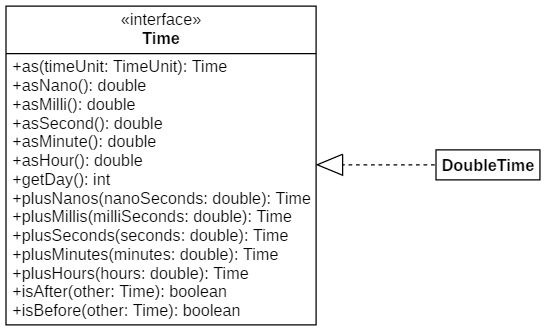
\includegraphics{figures/time.png}
    \caption[Time representation in DingNet simulator]{Time representation that provides all the basic functionalities.}
    \label{fig:time}
\end{figure}

\subsection{Communication protocol between mote and gateway}
%  communication protocol mote-gateway (interface sender and receiver).
In the LoRaWAN protocol every mote can start a transmission at every time based on its needs, without checks the transmission medium (ALOHA-like protocol).
Actually the simulator encapsulates this behaviour inside the class \mbox{\textit{NetworkEntity}}, that is the base class for \mbox{\textit{Gateway}} and \mbox{\textit{Mote}}. 
This architecture is modified with the new one presented in \autoref{fig:sendRec}. 
The new architecture generalizes the behaviour and it allows to evaluate the network behaviour with several variants of ALOHA-like protocol.
\mbox{\textit{Sender}} interface defines methods to send a packet, check the transmission status, and manage parameters that influence the transmission; while the \mbox{\textit{Receiver}} interface defines methods to receive incoming transmissions, and allows to the \mbox{\textit{NetworkEntity}} to specify how manage them.
\begin{figure}[h]
    \centering
    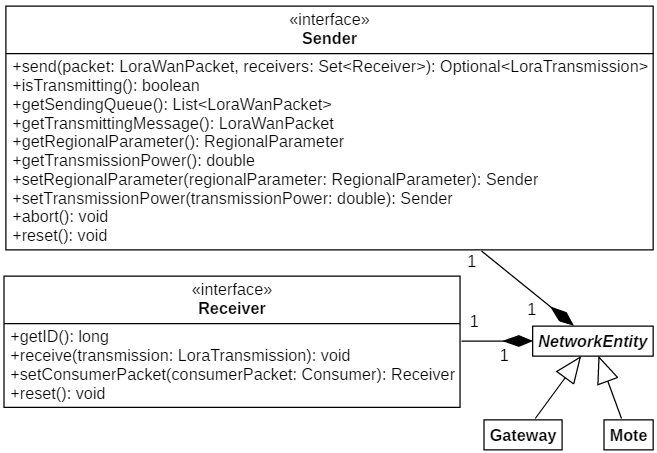
\includegraphics{figures/sendRec.png}
    \caption{\mbox{\textit{NetworkEntity}} architecture with \mbox{\textit{Sender}} and \mbox{\textit{Receiver}} interfaces.}
    \label{fig:sendRec}
\end{figure}

\subsection{Managing of incoming message to a LoRa mote}
The LoRaWAN protocol allows communication from gateways to motes, also if it is discourage for physical limitation of the transmission medium. 
The simulator partially supports this communication: it is designed only the structure to manage \textit{MAC Commands} (special commands exchange between network server and motes for network administration) motes side.
To complete the managing of incoming messages to a LoRa mote, allowing to use all the information presents in the payload, the architecture presented in \autoref{fig:consume} is designed.
\mbox{\textit{ReceivedPacketStrategy}} defines the strategy to use to store all the incoming packets and manage the pending queue of packets to consume.
\mbox{\textit{ConsumePacketStrategy}} defines how use the information in the payload to produce a side-effect on the LoRa mote or on the environment. 
Every mote can have a list of \mbox{\textit{ConsumePacketStrategy}}, which are performed in an ordered way with strategy that can use or ignore the packet.
\autoref{fig:consume} shows two implementation for the \mbox{\textit{ReceivedPacketStrategy}}, and none for \mbox{\textit{ConsumePacketStrategy}}. This because the first strategies are cross domain while the second ones are domain specific in respect of the simulated application.
\begin{figure}[h]
    \centering
    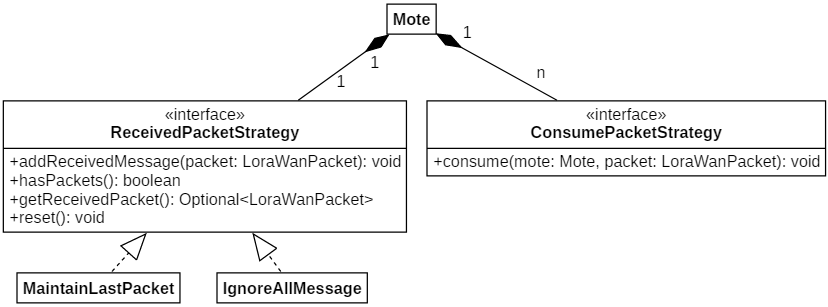
\includegraphics[width=\textwidth]{figures/consumePacket.png}
    \caption{Architecture to manage incoming packets mote side}
    \label{fig:consume}
\end{figure}

\subsection{Communication between Gateways and Applications}
In a LoRa-over-MQTT network, communications between gateways and applications are MQTT based and intermediated by the network server.
Actually in the simulator missing both the network server and the MQTT communication. 
So to simulate in a batter way the network's behaviour it is necessary to implements both.

\subsubsection{MQTT communication}
In addition to emulating the MQTT behaviour, the following requirements for the MQTT client have been defined:
\begin{itemize}
    \item[Req1.] allow simulations with different client abstractions, optimizations, and realize a simulator technology independent for MQTT client's implementation 
    \item[Req2.] avoid MQTT messages conversions to domain specific objects at each topic \mbox{subscription}.
\end{itemize}
To fulfill Req1 it is necessary to allow to switch client implementation in a simple and fast way (for example from a mock implementation to a real one).
To do so it has been defined the interface \mbox{\textit{MqttClient}}, avoiding to use directly a particular implementation.
It represents a MQTT client and it provides all the basic functionalities to interact with a MQTT broker. 
This interface allows to use custom implementations of MQTT client or external libraries implementing a wrapper extending the interface.
% 
To satisfy Req2 it is necessary to delegate conversions from and to the MQTT message type to the client, which interacts with the broker and knows how manipulates them.
% 
This requires to specify the receiving message type during the topic subscription phase.
% 
\autoref{fig:mqtt} shows the \mbox{\textit{MqttClient}} interface and its actual available implementations.
\begin{figure}[h]
    \centering
    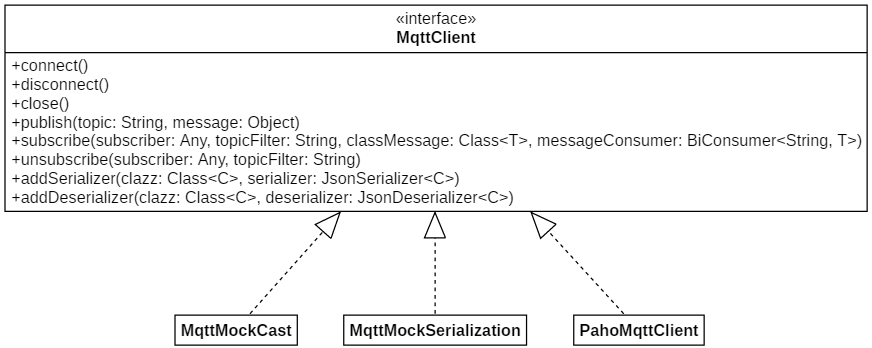
\includegraphics[width=\textwidth]{figures/mqttClient.png}
    \caption[\textit{MqttClient} interface and its available implementations]{\textit{MqttClient} interface and its available implementations. Thanks to \mbox{\textit{addSerializer}} and \mbox{\textit{addDeserializer}} methods it is possible to define custom strategies to convert messages for each client.}
    \label{fig:mqtt}
\end{figure}

\noindent The designed architecture is not valid only for this project, but it is reusable in different project, so it is decided to export it as external library. The library is actually available on github\footnote{\href{https://github.com/Placu95/MqttClientWrapper}{https://github.com/Placu95/MqttClientWrapper}} and a release on Maven Central Repository is planned shortly.

\subsubsection{Network server}
The network server is the entity appointed to regulate the communication between gateways and applications, but there isn't any specification that define which tasks has to perform and which is its architecture. 
Different providers propose different solutions. 
The solution designed for the simulator is composed from an autonomous simulator entity and performs two tasks:
\begin{enumerate}
    \item filtering of duplicated messages in communication from gateways to applications
    \item selections of the best gateway to deliver an application's message to a LoRa mote. 
    Default strategy to choose the gateway selects the gateway that has received the last transmission from the LoRa mote with more transmission power, but it is possible to change it defining different strategies. 
\end{enumerate}
\autoref{fig:GtoA} presents the new communication schema from a gateway, which receives a LoRa transmission, to the application; while \autoref{fig:AtoG} presents the new communication schema from an application, which wants to send a message to a LoRa mote, to the selected gateway that performs the LoRa transmission.
\begin{figure}[h]
    \centering
    \begin{subfigure}{.495\textwidth}
        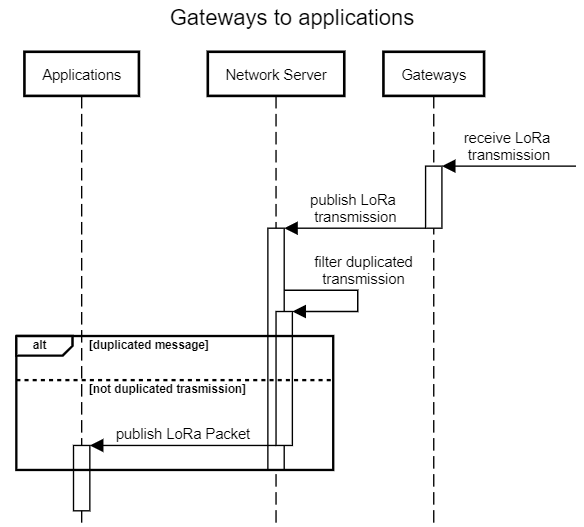
\includegraphics[scale=0.37]{figures/GtoApp.png}
        \caption{Communication from gateways \\to application}
        \label{fig:GtoA}
    \end{subfigure}
    \begin{subfigure}{.495\textwidth}
        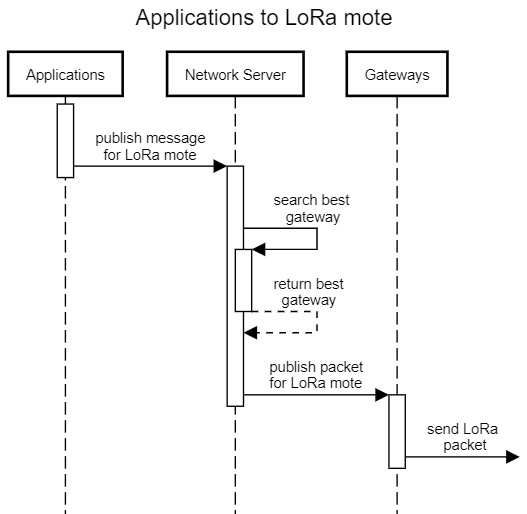
\includegraphics[scale=0.37]{figures/AppToG.png}
        \caption{Communication from application \\to gateways}
        \label{fig:AtoG}
    \end{subfigure}
    \caption{Communications between gateways and applications}
    \label{fig:netSer}
\end{figure}

\subsection{Timed run}
The simulator allows to execute two types of simulations: single run simulations and multiple run simulations, which consist simply in run more time a single run simulation. 
A single run simulation finishes when all the mobile LoRa motes arrive to the respective destination. 
This behaviour is limiting because it is impossible execute simulations with only fixed LoRa mote or simulations that continue also after then every mote is arrived to destination. 
To go beyond these limitations a new type of simulation is introduced: the \textit{Timed run} simulation. 
This type of simulation differs from the single run only for the termination condition. 
The condition requires to define the duration of the simulation, so the condition evaluates it as finished when the defined time is passed.

\subsection{Ranged sensor}
The DingNet simulator was developed to simulate self-adaptative applications based on received LoRa transmissions, so until now the real content of LoRa packet's payload was ignored.
The behaviour of different kinds of applications could instead depend from the payload. 
The idea is to define a new type of sensor that produces values in a configurable way splitting the region of simulation in a matrix of configurable dimension. 
So for each cell of the matrix it is defined a list configurations. 
Each cell's configuration defines the starting time of validity and the range of producible values. 
Then starting from this configuration is produced a tricubic spline interpolation function where the three variable are: the two coordinates of the matrix and the time; while the result is the corresponding sensor value.
Finally, when a mote requires a new value to the the sensor, it produces the value considering the mote position and the simulation time.
The result is that each sensor inside the same cell produces the same value at the same time. 
The architecture of this sensor is presented in \autoref{fig:rangedSensor}, where:
\begin{itemize}
    \item \textbf{SensorDataGenerator} $\rightarrow$ is the basic interface for sensors, it is already present in the simulator
    \item \textbf{Cell} $\rightarrow$ is the representation of the cells that compose the configurable matrix
    \item \textbf{RangeValue} $\rightarrow$ is the range of validity for the value to produce
    \item \textbf{RangeDataGenerator} $\rightarrow$ is the abstract class that loads the configuration file of the sensor, generates the interpolating function and produces values for LoRa motes. It requires only to define the type of the two interfaces \textit{Cell} and \textit{RangeValue}.
\end{itemize}
% 
\begin{figure}[h]
    \centering
    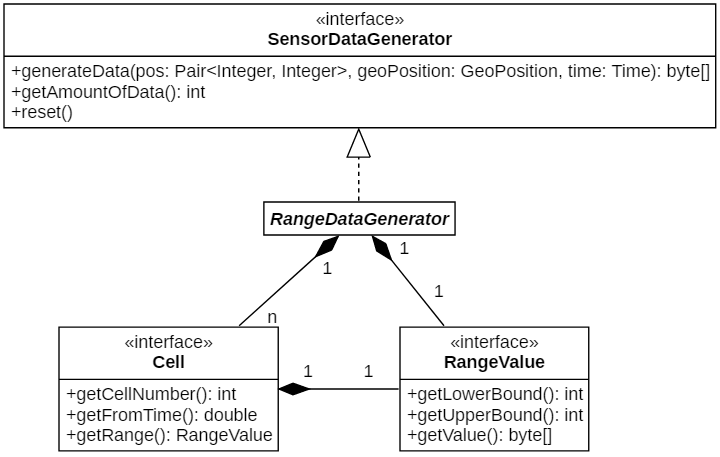
\includegraphics[scale=0.7]{figures/rangedSensor.png}
    \caption{Architecture of the configurable sensor}
    \label{fig:rangedSensor}
\end{figure}
% 
The actual file format for the sensor configuration file is \textit{toml}\footnote{\href{https://github.com/toml-lang/toml}{https://github.com/toml-lang/toml (Feb 2020)}}, but thanks to the \textit{konf}\footnote{\href{https://github.com/uchuhimo/konf}{https://github.com/uchuhimo/konf (Feb 2020)}} library (used to parse the file) it will be possible to change the file format with low effort.



\section{Aggregate programming over a LoRa-over-MQTT network}
\label{sec:contributionACOverDingNet}
This section discusses the integration between the aggregate computing paradigm and a LoRa-over-MQTT network like DingNet; enabling the simulation of aggregate applications on this platform.
In order to join these two concepts, first is necessary to define how map the networks entities in an aggregate computing system, and second identifies potentially additional requirements or limitations for these entities.
In the aggregate computing viewpoint, a system is composed of a set of distributed heterogeneous computational entities, called nodes. Nodes execute the same global program and communicate with a subset of them defined by a neighbourhood policy. 
While, in a LoRaWAN network the main entities are: LoRa motes, gateways, and network server; but at application level the only interesting entities are the LoRa motes.
So, following the aggregate vision it is natural to map each LoRa mote in a node that represents its digital twin (from now on called LoRa node) inside the aggregate system.
\\On the one hand, LoRa nodes can be considered as generic nodes and they do not require any specific neighbourhood's policy, or the use of particular communication technology to interact with their neighbours. 
But on the other hand, they have to support communication via MQTT to enable bidirectional communication with the respective physical counterparts.
Finally, it is necessary to analyse if all the network entities, or only some of them, can host the aggregate nodes.
In \cite{CCNCPS2018} the authors present a software architecture to enable the execution of aggregate computing programs on LoRa motes, but after evaluations of the proposed solution, they identify some issues due to the physical limitations of the communication technology. 
These issues do not allow to execute aggregate computing program directly on the LoRa motes, but they are not valid for the others network entities and there is any paper that identifies others possible issues.
Even if all the LoRaWAN network entities excluded the motes can host the aggregate node (LoRa nodes or others types of nodes), it is important to specify a limitation for the LoRa nodes. 
The LoRa nodes can interact with the respective LoRa mote only following the interaction schema defined from the LoRa-over-MQTT networks. 
For example, if a LoRa node is hosted by a LoRa gateway, that receives directly the transmissions of the respective LoRa mote, it cannot receive directly the packet, but it has to wait that the packet is published on the MQTT broker.

\subsection{Integration of Protelis with DingNet}
\label{sec:PoverD}
% The following subsection presents the software architecture designed to support the LoRa nodes inside an aggregate computing system defined in \textit{Protelis}.
The only things to do to enable the develop of Protelis applications over the DingNet network is to satisfy the requirement previously identified.
That requirement represents a specific capability of this type of nodes and Protelis defines a single place appointed to host it, the \mbox{\textit{ExecutionContext}}.
\autoref{fig:execContext} shows the model of the \mbox{\textit{ExecutionContext}} designed for the LoRa nodes. 
\begin{figure}[H]
    \centering
    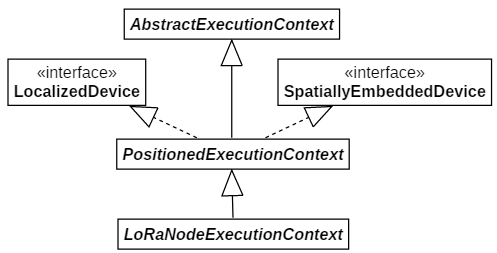
\includegraphics{figures/execContext.png}
    \caption{Model of \textit{ExecutionContext} for LoRa nodes}
    \label{fig:execContext}
\end{figure}
\noindent For devices spatially embedded and mainly used to transmit sensor values, their position is a relevant information. So, \mbox{\textit{PositionedExecutionContext}} is defined, which extends \mbox{\textit{AbstractExecutionContext}} (provided by Protelis) implementing the two interfaces that define functions to obtain spatial information of the device.
\mbox{\textit{LoRaNodeExecutionContext}} is the basic execution context for a LoRa node that:
% 
\begin{itemize}
    \item adds support for MQTT communication, satisfying the identified requirement
    \item encapsulates the subscription to the MQTT topic to receive the sensed values from the respective LoRa mote
    \item manages the received packet adding the sensed values to the knowledge-based of the node, or modifying its position if the value belongs to the GPS sensor.
\end{itemize}
% 
The introduced model enables the design of Protelis application composed of LoRa nodes, but also of not LoRa nodes.
Protelis applications with the model presented in \autoref{fig:appP} are not only valid for the DingNet network but for all the LoRa-over-MQTT networks that provide LoRa mote's data on a MQTT broker.
% 
\begin{figure}[H]
    \centering
    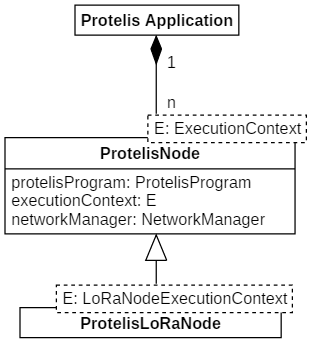
\includegraphics{figures/app.png}
    \caption{Abstract model of a Protelis application composed of LoRa nodes}
    \label{fig:appP}
\end{figure}
% 
\noindent In order to execute Protelis applications on the top of DingNet simulator, enabling the simulation of Protelis applications composed of LoRa nodes, is necessary one last small operation: unify the concept of time. 
This operation is necessary because the behaviour of every Protelis node depends also from the time in which their execution is scheduled, and the LoRa packets are received.
To do this it is sufficient wrapping the \mbox{\textit{LoRaNodeExecutionContext}} using the simulator time concept.

\paragraph{Concluding.} This chapter has presented the main works done during this thesis. First it has presented the improvements and evolution of the DingNet simulator model. Then it has presented the support to simulate Protelis application inside the DingNet simulator. \todo{TODO}